Rancangan variabel kepentingan akan dilakukan dengan menggunakan metode Random Forest. Metode Random Forest akan menghasilkan variabel kepentingan yang dapat dilihat pada Gambar \ref{fig:variabel-kepentingan}. Variabel kepentingan ini akan digunakan untuk melakukan analisis risiko autentikasi.
Berikut adalah rancangan variabel kepentingan yang akan digunakan untuk melakukan analisis risiko autentikasi.
\begin{figure}[H]
    \centering
    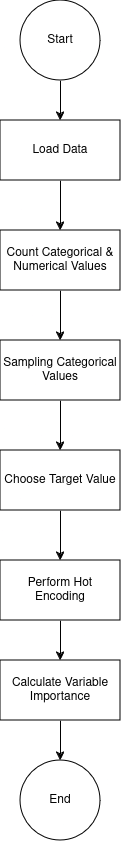
\includegraphics[width=0.2\textwidth]{BAB_TESIS/IMAGES/vim_1.drawio.png}
    \caption{Rancangan Variabel Kepentingan}
    \label{fig:variabel-kepentingan}
\end{figure}

Gambar \ref{fig:variabel-kepentingan} menggambarkan proses analisis data secara struktural yang digunakan dalam pengolahan data untuk tujuan tertentu. Proses dimulai dengan memuat data \textit{(Load Data)} yang akan digunakan dalam analisis. Setelah data dimuat, langkah berikutnya adalah menghitung nilai kategorikal dan numerik dalam dataset \textit{(Count Categorical \& Numerical Values)} guna memahami distribusi serta tipe data yang ada.

Setelah nilai-nilai tersebut dihitung, proses berlanjut dengan pengambilan sampel nilai kategorikal \textit{(Sampling Categorical Values)}. Pengambilan sampel ini bertujuan untuk memperoleh representasi yang lebih seimbang dan bermakna dari kategori yang ada dalam dataset. Kemudian, target value yang akan dianalisis ditentukan \textit{(Choose Target Value)}, yang menjadi fokus utama dalam proses analisis data lanjutan.

Langkah selanjutnya adalah melakukan penyandian hot encoding (Perform Hot Encoding) pada nilai kategorikal. Hot encoding adalah teknik yang mengubah berbagai nilai kategorikal menjadi format numerik biner, sehingga bisa digunakan dalam algoritma pembelajaran mesin. Setelah proses hot encoding selesai, tahapan berikutnya adalah menghitung tingkat pentingnya variabel \textit{(Calculate Variable Importance)}. Ini merupakan analisis untuk mengidentifikasi variabel mana yang paling berpengaruh terhadap target value yang telah dipilih sebelumnya.

Akhirnya, setelah seluruh proses perhitungan dan penyandian selesai, proses berakhir (End), menandakan bahwa data telah siap untuk tahap analisis atau pemodelan lebih lanjut.